\chapter{Introduction}
\label{chap:introduction}

\section{Initial Situation}
Digital Twins are a key technology at the very front of the fourth industrial revolution, coined Industry 4.0.
Latter term is characterized by the convergence of cyber-physical systems (CPS), the Internet of Things (IoT), and cloud computing to create smart factories with the goal of automation and efficiency \parencite{Oztemel2020}. An important concept within Industry 4.0 is the digital twin (DT). It can be defined as a virtual representation of physical assets enabling real-time monitoring and optimization \parencite{Tao2018ijamt}. The twin is an enabling technology, bridging the connection between the two entities with a bi-directional data flow to exchange information and to influence the behaviour of the physical asset \parencite{grieves2014digital}. This technology in Industry 4.0 connects the physical and digital worlds through real-time data integration, simulation, and optimization \parencite{judijanto2024trends}.

Although this field is rapidly evolving, there has not been found a common ground about the definition of DT. The term was first introduced by Michael Grieves in 2002, defining it as a digital representation of a physical object or system \parencite{grieves2014digital}. However, the concept has evolved since then, encompassing a broader range of applications and technologies. Going back through the literature, there are three words for describing similar characteristics of DT: Digital Model (DM), Digital Shadow (DS) and Digital Twin (DT) \parencite{jones2020characterising,Zhang2021jmsy}.

\begin{figure}[htbp]
  \centering
  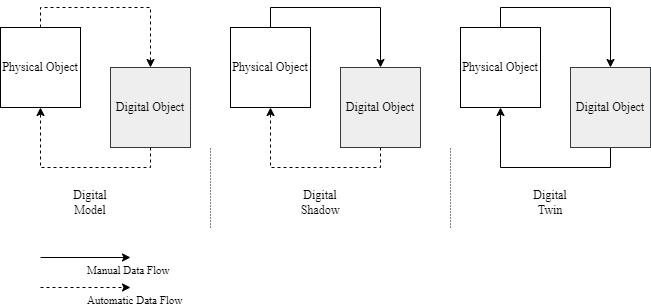
\includegraphics[width=0.8\textwidth]{figures/kritzinger.png}
  \caption{Comparison of Digital Shadow (DS), Digital Model (DM) and Digital Twin (DT) as presented by Kritzinger.}
  \label{fig:Kritzinger}
\end{figure}

The DM simply contains manual data connections between physical and digital entities. These connections can be temporarily shifted or even disconnected. There is no control of the digital object over the physical entity. It rather is a simple or complex model \textit{describing} the modelled object. It can not make decisions by itself to influence the physical object. The reason lies in the potential outdated data the digital part posesses or in the fact that it can not trigger the data flow back to the physical part by itself. The control is completely in the hands of the modeller.
The DS is a more advanced version of the DM. It is a digital representation of the physical object, which is continuously updated with real-time data. The DS can be used for monitoring, analysis and simulation purposes. It can predict the future state of the physical object based on the current state and historical data. However, the DS is not able to influence the physical object. The control is, similar to the DM, still in the hands of the modeller. A DS is mainly used for simulation and in the literature often confusingly classified as a DT. The DT is the most advanced version of the three. It is a digital representation of the physical object, which is alos continuously updated with real-time data. The DT can be used for monitoring, analysis, and control purposes. It can predict the future state of the physical object based on the current state and historical data. The DT can also influence the physical object by sending control signals to it. The control is partially or completely in the hands of the DT. The DT thus \textit{can} serve more purpoose than modelling or simulating the physical object. It may serve as an autonomic system, updating itself or by help of the modeller \parencite{kritzinger2018digital}.

Transitioning to Industry 5.0, there is a paradigm shift placing humans at the center of technological advancements, emphasizing collaboration between humans and machines for a more personalized, sustainable, and resilient manufacturing environment \parencite{Davim2023}. Industry 5.0 seeks to harmonize technological progress with human values and sustainability, moving beyond the efficiency focus of Industry 4.0 \parencite{Espina-Romero2023}. Digital twins remain crucial in Industry 5.0, facilitating a human-centric approach by serving as adaptive models that integrate data between physical and virtual entities, supporting complex knowledge management \parencite{Chryssolouris2024}.

In essence, while both Industry 4.0 and 5.0 utilize digital twins, their core focus diverges. Industry 4.0 prioritizes technological integration and efficiency \parencite{Lu2020}, whereas Industry 5.0 emphasizes human-centric values and sustainable practices \parencite{Leng2023}. This evolution reflects a broader societal shift towards aligning technological progress with human and environmental well-being.

\section{Problem}
% Content goes here

\section{Objective of the Thesis}
% This section includes: Motivation, Relevance, Research Questions, and Hypotheses
% Content goes here

\section{Structure of the Thesis and Methodological Approach}
% Content goes here

\chapter{Introduction}

Diese Arbeit befasst sich mit der automatisierten Verifikation und Validierung von automatisiert generierten, simulationsbasierten digitalen Zwillingen für diskrete Materialflusssysteme. Im Zuge der Digitalisierung industrieller Prozesse und der vierter industriellen Revolution (Industrie 4.0) gewinnen digitale Zwillinge zunehmend an Bedeutung. Die vorliegende Einleitung skizziert zunächst die aktuelle Situation und den daraus resultierenden Bedarf, formuliert das zentrale Problem sowie die Zielsetzung der Arbeit und erläutert abschließend den Aufbau sowie die methodische Vorgehensweise.

\section{Initial Situation}

Im Rahmen der vierten industriellen Revolution findet eine verstärkte Integration von Informations- und Kommunikationstechnologien in Produktions- und Logistikprozesse statt. Digitale Zwillinge, also virtuelle Repliken physischer Systeme, ermöglichen nicht nur die Überwachung von Anlagen, sondern auch deren dynamische Simulation und Optimierung. Besonders in diskreten Materialflusssystemen – wie sie in der Automobilindustrie, der Logistik oder in hochautomatisierten Fertigungsprozessen vorkommen – erweist sich die präzise Modellierung von Materialflüssen als Schlüsselfaktor für Effizienz und Wettbewerbsfähigkeit \parencite{Grieves2014}.

Die rasante Entwicklung im Bereich der Sensorik und des Internet of Things (IoT) liefert kontinuierlich große Datenmengen, die in digitalen Zwillingen genutzt werden können, um den aktuellen Zustand von Produktionssystemen nahezu in Echtzeit abzubilden. Traditionelle Simulationsansätze, die oft auf statischen Modellen basieren, werden durch die dynamische Natur digitaler Zwillinge ergänzt, die durch kontinuierliche Datenintegration eine verbesserte Prozesssteuerung und prädiktive Instandhaltung ermöglichen \parencite{Tao2018}. Dabei stellen digitale Zwillinge eine Schnittstelle zwischen der realen und der virtuellen Welt dar und bieten somit die Möglichkeit, komplexe industrielle Abläufe zu überwachen, zu simulieren und zu optimieren.

Die zunehmende Digitalisierung und Vernetzung führen jedoch auch zu neuen Herausforderungen. Die Komplexität moderner Systeme sowie die enorme Datenflut erfordern innovative Ansätze zur Modellierung und kontinuierlichen Aktualisierung. Hierbei steht insbesondere die automatisierte Generierung von Simulationsmodellen im Vordergrund, die durch datengetriebene Verfahren unterstützt wird. Dieser Paradigmenwechsel fordert nicht nur traditionelle Simulationsmethoden heraus, sondern eröffnet auch neue Perspektiven für die industrielle Praxis, indem er die Grundlage für eine optimierte Entscheidungsfindung schafft \parencite{Uhlemann2017}.

\section{Problem}

Trotz des hohen Potenzials digitaler Zwillinge treten in der Praxis zahlreiche Herausforderungen auf. Die automatisierte Erstellung simulationsbasierter Modelle birgt das Risiko, dass wesentliche Systemkomponenten oder Interaktionsmuster unzureichend erfasst werden. Dies führt zu Diskrepanzen zwischen dem digitalen Modell und dem realen System, was im schlimmsten Fall die Grundlage für fehlerhafte Simulationen und falsche betriebliche Entscheidungen bildet. Traditionelle Verifikations- und Validierungsprozesse (V\&V) basieren häufig auf manuellen Prüfungen, die angesichts der Komplexität und der Datenmengen in modernen Produktionssystemen nicht mehr effizient durchführbar sind \parencite{Kritzinger2018}.

Ein weiteres Problemfeld stellt die Integration von Echtzeitdaten in die Simulationsmodelle dar. Während historische Daten die Basis statischer Modelle bilden, erfordert die dynamische Anpassung digitaler Zwillinge die kontinuierliche Auswertung und Synchronisation aktueller Betriebsdaten. Dies führt zu Herausforderungen hinsichtlich der Datenkonsistenz, -qualität und -verarbeitung. Zudem fehlt es oft an standardisierten Bewertungsmetriken, die eine objektive Beurteilung der Modellgüte ermöglichen. Diese Probleme machen deutlich, dass herkömmliche V\&V-Methoden nicht ohne Weiteres auf automatisiert generierte, simulationsbasierte digitale Zwillinge übertragbar sind.

Insbesondere in diskreten Materialflusssystemen, in denen zahlreiche Prozessvariablen und Interaktionskomponenten eine Rolle spielen, erfordert die Sicherstellung der Modellgenauigkeit neue Ansätze. Es besteht daher dringender Forschungsbedarf, um datengetriebene und automatisierte V\&V-Methoden zu entwickeln, die den spezifischen Anforderungen solcher Systeme gerecht werden \parencite{Kritzinger2018, Uhlemann2017}.

\section{Objective of the Thesis}

Das Hauptziel dieser Arbeit ist die Entwicklung eines datengetriebenen Frameworks zur automatisierten Verifikation und Validierung von digital generierten, simulationsbasierten digitalen Zwillingen. Der Fokus liegt dabei auf diskreten Materialflusssystemen, da diese aufgrund ihrer Komplexität und Dynamik besondere Herausforderungen hinsichtlich der Modellgenauigkeit und Prozesssynchronisation aufweisen.

\subsection*{Motivation und Relevanz}

Die Motivation dieser Forschungsarbeit ergibt sich aus mehreren zentralen Aspekten:
\begin{itemize}
  \item \textbf{Effizienzsteigerung:} Durch den Einsatz automatisierter V\&V-Methoden können Modellabweichungen frühzeitig erkannt und behoben werden, was zu einer signifikanten Reduktion von Fehlerquellen und Optimierungspotenzialen in Produktionsprozessen führt.
  \item \textbf{Digitalisierung und Vernetzung:} Mit der zunehmenden Integration von IoT und Sensorik in Produktionsanlagen steigt die Verfügbarkeit von Echtzeitdaten, die in digitalen Zwillingen verarbeitet werden können. Ein zuverlässiges V\&V-Framework stellt sicher, dass diese Daten adäquat in die Modelle einfließen.
  \item \textbf{Wettbewerbsvorteile:} Unternehmen, die in der Lage sind, ihre digitalen Modelle präzise und effizient zu validieren, sichern sich langfristig Wettbewerbsvorteile in einem zunehmend globalisierten Marktumfeld \parencite{Grieves2014}.
\end{itemize}

\subsection*{Forschungsfragen und Hypothesen}

Die Arbeit fokussiert sich auf folgende Forschungsfragen:
\begin{itemize}
  \item Wie können automatisierte Prozesse zur Verifikation und Validierung von digital generierten, simulationsbasierten digitalen Zwillingen effizient implementiert werden?
  \item Welche datengetriebenen Ansätze eignen sich am besten, um Abweichungen zwischen simuliertem Verhalten und realen Betriebsdaten in diskreten Materialflusssystemen zu identifizieren?
  \item Inwieweit verbessert das entwickelte Framework die Qualität und Zuverlässigkeit der digitalen Zwillinge im Vergleich zu traditionellen V\&V-Methoden?
\end{itemize}

Es wird die Hypothese aufgestellt, dass ein integriertes, datengetriebenes V\&V-Framework signifikante Verbesserungen in der Modellgenauigkeit und Effizienz der Validierungsprozesse bewirken kann. Durch den Einsatz moderner Datenanalysen und maschineller Lernverfahren sollen systematische Abweichungen frühzeitig erkannt und Korrekturmaßnahmen automatisiert eingeleitet werden \parencite{Tao2018}.

\section{Structure of the Thesis und Methodological Approach}

Der Aufbau dieser Arbeit gliedert sich in mehrere Kapitel, die im Folgenden kurz vorgestellt werden:

\begin{itemize}
  \item \textbf{Kapitel \ref{chap:literature}:} Umfassende Literaturrecherche. In diesem Kapitel werden die theoretischen Grundlagen digitaler Zwillinge, bestehende Simulationsansätze und aktuelle V\&V-Methoden analysiert.
  \item \textbf{Kapitel \ref{chap:framework}:} Entwicklung des datengetriebenen Frameworks. Hier werden die konzeptionellen und architektonischen Entscheidungen, die Auswahl der Algorithmen und die Implementierungsdetails dargestellt.
  \item \textbf{Kapitel \ref{chap:caseStudy}:} Fallstudie. Anhand eines konkreten Beispiels aus dem Bereich der diskreten Materialflusssysteme wird das entwickelte Framework empirisch validiert.
  \item \textbf{Kapitel \ref{chap:evaluation}:} Evaluation. Die Ergebnisse der Fallstudie werden hinsichtlich Modellgenauigkeit, Prozesszeiten und Fehlerhäufigkeiten quantitativ und qualitativ ausgewertet.
  \item \textbf{Kapitel \ref{chap:conclusion}:} Zusammenfassung und Ausblick. Abschließend werden die wesentlichen Erkenntnisse zusammengefasst, Limitationen diskutiert und Perspektiven für zukünftige Forschungsarbeiten aufgezeigt.
\end{itemize}

Methodologisch basiert die Arbeit auf einem iterativen Entwicklungs- und Validierungsansatz, der sowohl qualitative als auch quantitative Methoden integriert. Zunächst erfolgt eine detaillierte Literaturrecherche, um den aktuellen Stand der Technik zu erfassen und bestehende Forschungslücken zu identifizieren. Aufbauend auf diesen Erkenntnissen wird das Framework in modularer Form entwickelt. Die einzelnen Module – etwa für Datenerfassung, -vorverarbeitung, Modellgenerierung sowie die automatisierte V\&V – werden zunächst unabhängig implementiert und anschließend in ein Gesamtsystem integriert.

Ein zentraler Bestandteil der methodischen Vorgehensweise ist die empirische Validierung des Frameworks durch eine praxisnahe Fallstudie. Hierbei werden reale Prozessdaten eines diskreten Materialflusssystems herangezogen, um die Simulationsergebnisse kontinuierlich mit den tatsächlichen Betriebsdaten abzugleichen. Die Evaluation erfolgt durch die Analyse quantitativer Metriken (z. B. Abweichungsmaße, Reaktionszeiten) und wird durch qualitative Analysen ergänzt, um systemische Fehlerquellen aufzudecken \parencite{Uhlemann2017}.

Die Implementierung moderner Softwaretechnologien und datengetriebener Ansätze, wie etwa maschinelles Lernen, soll dabei helfen, die Validierungsprozesse zu automatisieren und flexibel an veränderte Betriebsbedingungen anzupassen. Der iterative Entwicklungsprozess ermöglicht es, das Framework kontinuierlich zu optimieren und auf die spezifischen Anforderungen unterschiedlicher industrieller Anwendungen zuzuschneiden. So wird ein dynamisches Instrument geschaffen, das nicht nur den theoretischen Anforderungen genügt, sondern auch in der Praxis anwendbar ist \parencite{Tao2018, Kritzinger2018}.

Zusammenfassend bietet diese Arbeit einen innovativen Beitrag zur Weiterentwicklung digitaler Zwillinge in diskreten Materialflusssystemen. Durch die Kombination theoretischer Fundierung, moderner datengetriebener Methoden und empirischer Validierung wird ein Framework vorgestellt, das signifikante Verbesserungen in der Modellgenauigkeit und Effizienz von V\&V-Prozessen ermöglicht. Die erzielten Ergebnisse tragen dazu bei, die Zuverlässigkeit digitaler Zwillinge zu erhöhen und bieten zugleich wertvolle Ansätze für die zukünftige Entwicklung in einer zunehmend digitalisierten und vernetzten Produktionslandschaft.
